\documentclass[11.5pt,twoside]{book}

% --------------------------------
% Page layout
% --------------------------------

\usepackage[
paperwidth=5.5in,
paperheight=8.5in,
top=0.85in,
bottom=0.85in,
inner=0.75in,
outer=0.6in,
headheight=14pt,
headsep=0.25in
]{geometry}

\usepackage[spanish]{babel}
\usepackage{microtype}

\tolerance=1000
\emergencystretch=3em
\hyphenpenalty=500
% --------------------------------
% Font
% --------------------------------
\usepackage{fontspec}
\setmainfont{Crimson Pro}

% --------------------------------
% Line spacing
% --------------------------------
\usepackage{setspace}
\setstretch{1.35}

% --------------------------------
% Microtypography
% --------------------------------
\usepackage{microtype}

% --------------------------------
% Images
% --------------------------------
\usepackage{graphicx}
\providecommand{\pandocbounded}[1]{#1}
% ----------------------------
% Images (Pandoc)
% ----------------------------

% Size of chapter sketches
\newcommand{\chapterillustration}{
\IfFileExists{images/ch\thechapter.png}{
\includegraphics[width=0.66\textwidth]{images/ch\thechapter.png}

\vspace{1em}
}{}
}

% Make images behave like inline content (no floating)
\usepackage{float}
\floatplacement{figure}{H}

% Fix Pandoc bounded images
% --------------------------------
% Headers
% --------------------------------
\usepackage{fancyhdr}

\pagestyle{fancy}
\fancyhf{}

\fancyhead[L]{\small LA IGLESIA CARNAL}
\fancyhead[R]{\small John Wry}

\fancyfoot[C]{\thepage}

% --------------------------------
% Paragraph style
% --------------------------------
\setlength{\parindent}{0pt}
\setlength{\parskip}{0.6em}

% --------------------------------
% Remove numbering
% --------------------------------
\setcounter{secnumdepth}{0}
\usepackage{pgfornament}
\usepackage{tikz}
\usetikzlibrary{shapes.geometric}
\newcommand{\chapterornament}{
\begin{center}
\pgfornament[width=3cm]{88}
\end{center}
}
% --------------------------------
% Chapter style
% --------------------------------
\newcommand{\chapterart}{
\IfFileExists{images/ch\thechapter.png}{
\begin{center}
\includegraphics[width=0.88\textwidth]{images/ch\thechapter.png}
\end{center}
\vspace{1em}
}{
\chapterornament
\vspace{1em}
}
}


\makeatletter
\renewcommand{\@makechapterhead}[1]{
\vspace*{3cm}

\begin{center}

{\Large\scshape Capítulo \thechapter}

\vspace{1em}

{\Huge\bfseries #1}

\vspace{1.2em}

\chapterart

\vspace{.5cm}

\end{center}

\vspace{0.2cm}
}
\makeatother



% --------------------------------
% Begin document
% --------------------------------
\begin{document}
\sloppy
% --------------------------------
% Cover
% --------------------------------

\begin{titlepage}
\thispagestyle{empty}

\newgeometry{margin=0pt}

\noindent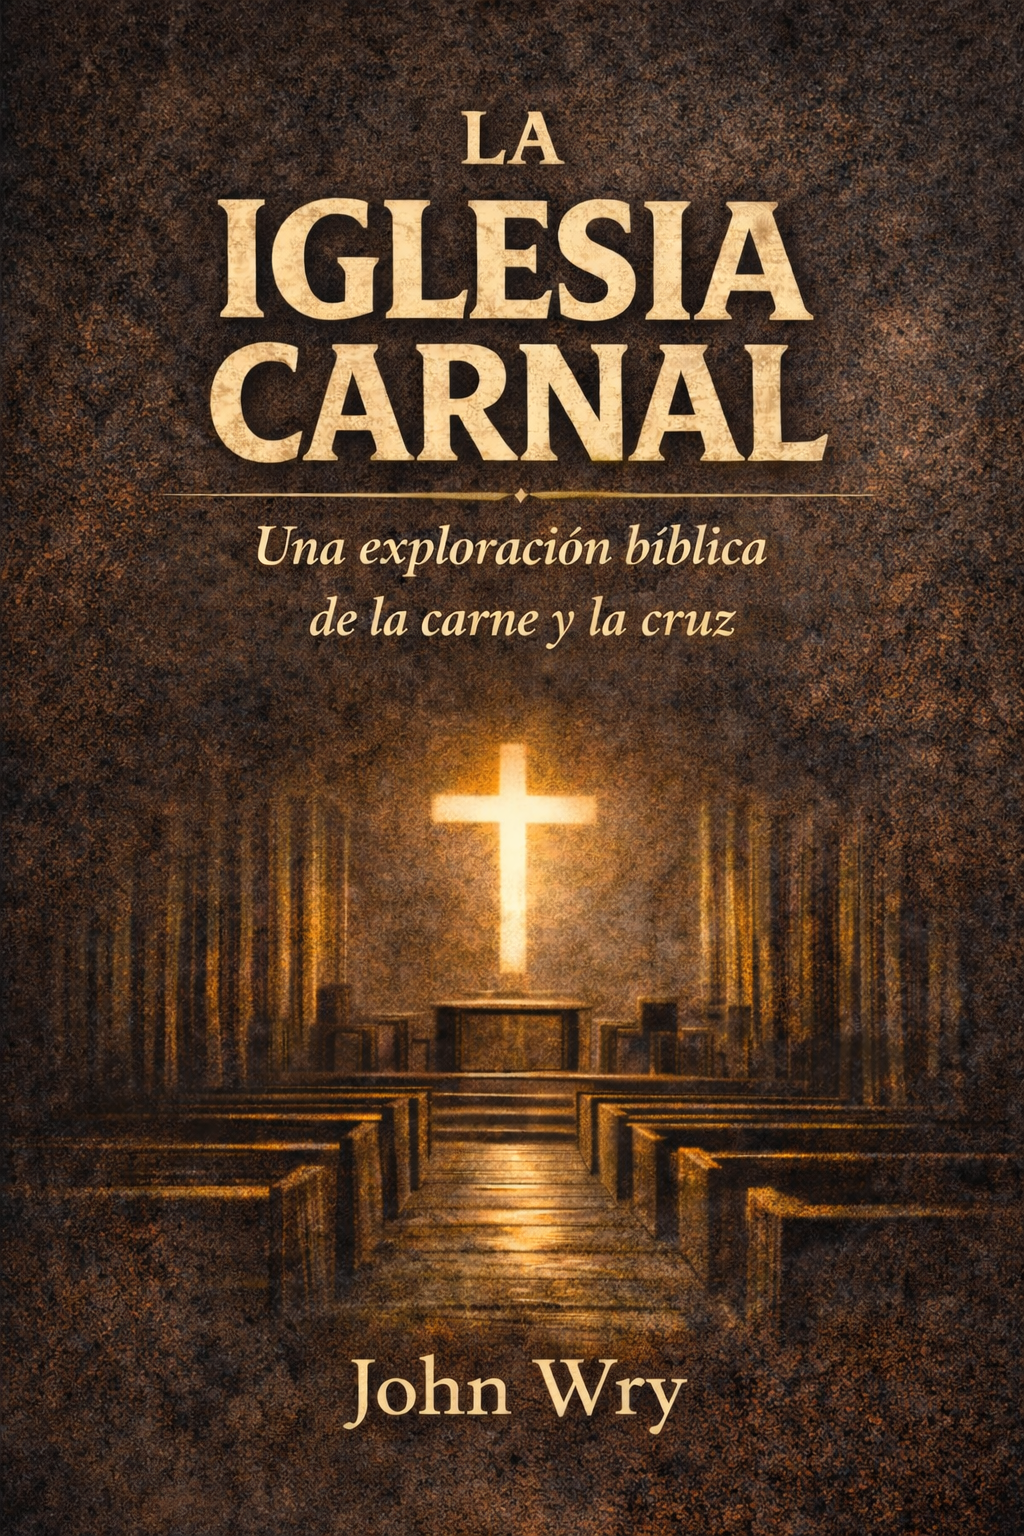
\includegraphics[
width=\paperwidth,
height=\paperheight
]{portada.png}

\restoregeometry
\end{titlepage}

% --------------------------------
% Title Page
% --------------------------------
\thispagestyle{empty}

\vspace*{3cm}

\begin{center}

{\Huge\bfseries La Iglesia Carnal}

\vspace{1cm}

{\Large Una exploración bíblica de la carne y la cruz}

\vfill

{\Large John Wry}

\end{center}

\clearpage

% --------------------------------
% Copyright Page
% --------------------------------
\thispagestyle{empty}

\vspace*{4cm}

\begin{center}
Primera edición\\
Derechos Reservados © 2026 John Wry

\vspace{1em}

Las citas bíblicas están tomadas de la
Biblia de las Américas (NBLA).

\vspace{1em}

Este libro puede compartirse libremente en formato digital,\\
siempre que no sea alterado.

\end{center}

\clearpage

% --------------------------------
% Dedication
% --------------------------------
\thispagestyle{empty}

\vspace*{4cm}

\begin{center}

Dedicado a mi esposa Nelly,
quien siempre ha estado a mi lado.\\

y\\

Para aquellos estudiantes \\
que se mantuvieron firmes en el evangelio\\
sin importar el costo.
\end{center}

\clearpage

% --------------------------------
% Table of Contents
% --------------------------------
\renewcommand{\contentsname}{Índice}
\tableofcontents

\clearpage

% --------------------------------
% Body
% --------------------------------
$body$

% --------------------------------
% Final Page
% --------------------------------
\clearpage
\thispagestyle{empty}

\vspace*{4cm}

\begin{center}

Gracias por leer.

\vspace{1cm}

Si este libro te ayudó, compártelo 
con alguien que esté lidiando con las mismas preguntas.\\

\vspace{1cm}

{\footnotesize
Algunas partes de este manuscrito fueron desarrolladas con la ayuda de herramientas
de lenguaje basadas en inteligencia artificial utilizadas para redacción, edición y
traducción. Todas las ideas, argumentos y conclusiones pertenecen al autor.
}

\end{center}

\end{document}